\chapter{Model sterowania ruchem drogowym}
TODO - tutaj opis ogólny modelu sterowania - sterowanie dyskretne, jakie czujniki co dają, co robi sygnalizator

TODO - co to są zakłócenia i jak wpływają na obiekt sterowany

\begin{figure}[h]
    \centering
    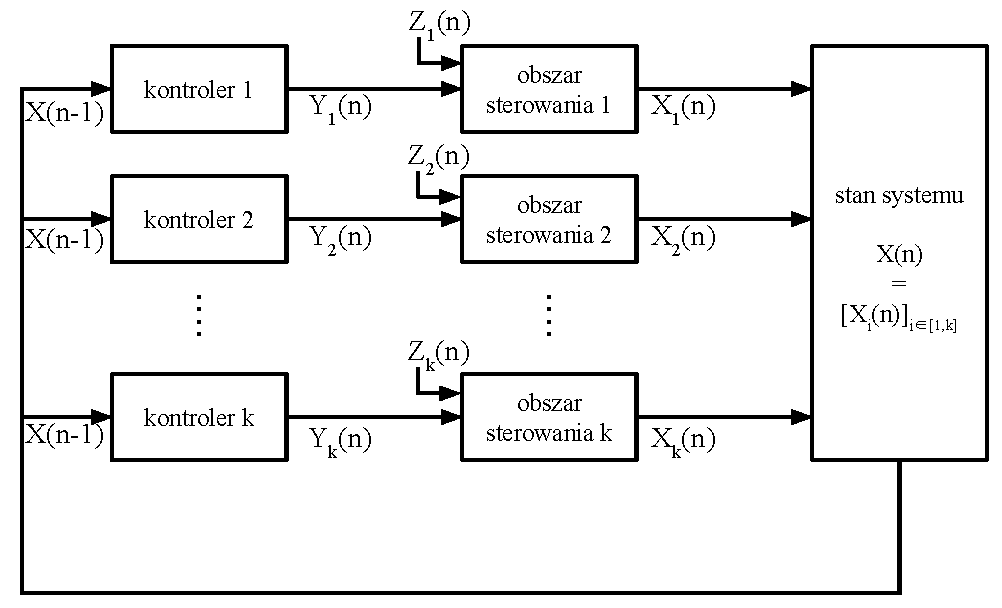
\includegraphics[width=0.8\textwidth]{images/model.pdf}
    \caption{Model systemu sterowania}
    \label{rys:model}
\end{figure}

Na rysunku \ref{rys:model} zaprezentowany został model sterowania ruchem drogowym.
Zespół skrzyżowań objęty sterowaniem podzielony jest na obszary.
Każdy obszar obejmuje pojedyncze skrzyżowanie lub jego autonomiczną część.
Autonomiczną, nazywamy część skrzyżowania, w której dojazd potoków ruchu do miejsca przecięcia nie jest kontrolowany
przez sygnalizatory nie znajdujące się w danej części skrzyżowania.

Każdy obszar sterowany jest przez pojedynczy kontroler.
Kontroler jako dane wejściowe przyjmuje stan systemu w poprzedniej chwili czasu,
który zawiera wielkości mierzone przez czujniki jak i sterowania wyznaczone przez wszystkie kontrolery.

TODO - ograniczenia sterowania -czasy itp

TODO - struktura sieciowa kontrolerów -kontrolery połączone przez sieć ethernet itp

TODO - wszystkie rzeczy z google drive